\documentclass[12pt,a4paper]{report}

% Encodage et langue
\usepackage[utf8]{inputenc}
\usepackage[T1]{fontenc}
\usepackage[french]{babel}

% Mise en page
\usepackage{geometry}
\geometry{left=2.5cm,right=2.5cm,top=2.5cm,bottom=2.5cm}
\usepackage{setspace}
\onehalfspacing

% Mathématiques
\usepackage{amsmath,amsfonts,amssymb}
\usepackage{amsthm}

% Graphiques et tableaux
\usepackage{graphicx}
\usepackage{float}
\usepackage{booktabs}
\usepackage{multirow}
\usepackage{array}
\usepackage{caption}
\usepackage{subcaption}
\graphicspath{{images/}}

% Code et algorithmes
\usepackage{xcolor}

% Hyperliens
\usepackage{hyperref}
\hypersetup{
    colorlinks=true,
    linkcolor=blue,
    filecolor=magenta,
    urlcolor=cyan,
    citecolor=blue
}

% En-têtes et pieds de page
\usepackage{fancyhdr}
\pagestyle{fancy}
\fancyhf{}
\fancyhead[L]{\leftmark}
\fancyhead[R]{\thepage}
\renewcommand{\headrulewidth}{0.4pt}

% Autres
\usepackage{enumitem}
\usepackage{url}

% Théorèmes et définitions
\theoremstyle{definition}
\newtheorem{definition}{Définition}[chapter]

% Informations du document
\title{\textbf{Prédiction Data-Driven de la Vie Utile Résiduelle (RUL)\\
appliquée au jeu de données CMAPSS de la NASA}}
\author{Rapport de Projet de Fin de Module}
\date{Année Universitaire 2025--2026}

\begin{document}

% ==================== PAGE DE GARDE ====================
\begin{titlepage}
    \centering
    \vspace*{1cm}
    
    {\Large \textbf{ÉCOLE D'INGÉNIEURS}}\\[0.3cm]
    {\large Nom de votre école}\\[1.5cm]
    
    \rule{\linewidth}{0.5mm}\\[0.6cm]
    {\Huge \bfseries Prédiction Data-Driven de la Vie Utile Résiduelle (RUL)}\\[0.3cm]
    {\LARGE \bfseries appliquée au jeu de données CMAPSS de la NASA}\\[0.2cm]
    \rule{\linewidth}{0.5mm}\\[1.5cm]
    
    {\Large \textit{Rapport de Projet de Fin de Module}}\\[1cm]
    
    \vfill
    
    \begin{minipage}{0.45\textwidth}
        \begin{flushleft}
            \textbf{Réalisé par :}\\
            Votre Prénom Nom
        \end{flushleft}
    \end{minipage}
    \hfill
    \begin{minipage}{0.45\textwidth}
        \begin{flushright}
            \textbf{Encadrant :}\\
            Nom de l'encadrant
        \end{flushright}
    \end{minipage}
    
    \vspace{1cm}
    {\large \textbf{Date de soutenance :} Date}\\[0.5cm]
    {\large Année Universitaire 2025--2026}
    
\end{titlepage}

% ==================== RÉSUMÉ ====================
\chapter*{Résumé}
\addcontentsline{toc}{chapter}{Résumé}

Ce rapport présente une étude de prédiction de la \emph{Vie Utile Résiduelle} (Remaining Useful Life, RUL) appliquée au jeu de données public \textsc{CMAPSS} (Commercial Modular Aero-Propulsion System Simulation) fourni par la NASA. L'objectif est de comparer l'efficacité de deux approches data-driven : une méthode classique d'apprentissage automatique fondée sur le gradient boosting (XGBoost) et une méthode d'apprentissage profond basée sur les réseaux de neurones récurrents de type LSTM (Long Short-Term Memory).

Le travail s'appuie sur trois notebooks Jupyter détaillant respectivement le prétraitement des données, la conception du modèle XGBoost et celle du modèle LSTM. Les résultats expérimentaux montrent que le modèle LSTM surpasse le modèle XGBoost sur le sous-ensemble FD001, avec une erreur quadratique moyenne (RMSE) de 15,17 contre 19,07 cycles. Une application de démonstration basée sur Streamlit est également proposée pour illustrer les capacités de prédiction du modèle en temps réel.

\vspace{0.5cm}
\noindent\textbf{Mots-clés :} Vie Utile Résiduelle, RUL, maintenance prédictive, CMAPSS, XGBoost, LSTM, réseaux de neurones récurrents, apprentissage profond, pronostics.

\chapter*{Abstract}
\addcontentsline{toc}{chapter}{Abstract}

This report presents a study on Remaining Useful Life (RUL) prediction applied to the public NASA CMAPSS (Commercial Modular Aero-Propulsion System Simulation) dataset. The objective is to compare the effectiveness of two data-driven approaches: a classical machine learning method based on gradient boosting (XGBoost) and a deep learning method based on Long Short-Term Memory (LSTM) recurrent neural networks.

The work relies on three Jupyter notebooks detailing data preprocessing, XGBoost model design, and LSTM model design, respectively. Experimental results show that the LSTM model outperforms the XGBoost model on the FD001 subset, with a Root Mean Square Error (RMSE) of 15.17 versus 19.07 cycles. A Streamlit-based demonstration application is also proposed to illustrate the model's real-time prediction capabilities.

\vspace{0.5cm}
\noindent\textbf{Keywords:} Remaining Useful Life, RUL, predictive maintenance, CMAPSS, XGBoost, LSTM, recurrent neural networks, deep learning, prognostics.

% ==================== TABLE DES MATIÈRES ====================
\tableofcontents
\listoffigures
\listoftables

% ==================== INTRODUCTION ====================
\chapter{Introduction générale}

\section{Contexte et motivation}

Dans les domaines industriels à forte intensité capitalistique tels que l'aéronautique, l'énergie et les transports, la fiabilité des équipements critiques constitue un enjeu stratégique majeur. Une défaillance imprévue d'un composant essentiel peut entraîner des arrêts de production coûteux, voire des conséquences catastrophiques sur la sécurité des personnes et des biens. La maintenance prédictive, qui vise à anticiper les défaillances avant qu'elles ne surviennent, représente ainsi une évolution déterminante par rapport aux stratégies de maintenance corrective ou préventive traditionnelles.

Au coeur de la maintenance prédictive se trouve le problème de la \emph{prédiction de la vie utile résiduelle} (Remaining Useful Life, RUL). Il s'agit d'estimer, à partir de l'état actuel d'un système, le nombre d'unités de temps (cycles, heures, kilomètres) restantes avant sa défaillance. Cette capacité de pronostic offre aux opérateurs industriels une fenêtre temporelle suffisante pour planifier les interventions de maintenance, optimiser la gestion des stocks de pièces de rechange et minimiser les temps d'arrêt.

\section{Présentation du projet}

Ce projet de fin de module s'inscrit dans le cadre de l'étude des méthodes \emph{data-driven} pour la prédiction de la RUL. Il repose sur le projet open-source \texttt{rul\_codes\_open} de Biswajit Sahoo, qui vise à produire des résultats reproductibles dans le domaine du condition monitoring. Nous nous concentrons spécifiquement sur le jeu de données CMAPSS (Commercial Modular Aero-Propulsion System Simulation) de la NASA, simulant la dégradation de moteurs d'avions turbofan.

L'originalité de notre travail réside dans la comparaison systématique de deux approches complémentaires :
\begin{itemize}
    \item Une approche classique de \emph{machine learning} fondée sur l'algorithme XGBoost (eXtreme Gradient Boosting), représentatif des méthodes d'ensemble à base d'arbres de décision.
    \item Une approche d'\emph{apprentissage profond} fondée sur les réseaux LSTM (Long Short-Term Memory), capables de capturer les dépendances temporelles long terme inhérentes aux données de dégradation.
\end{itemize}

\section{Objectifs du rapport}

Les objectifs de ce rapport sont les suivants :
\begin{enumerate}
    \item Présenter de manière rigoureuse le jeu de données CMAPSS et les étapes de prétraitement nécessaires à son exploitation.
    \item Décrire les architectures des modèles XGBoost et LSTM implémentés, ainsi que leurs protocoles d'entraînement respectifs.
    \item Comparer quantitativement les performances des deux modèles à l'aide de métriques standardisées (RMSE et S-score).
    \item Illustrer les résultats obtenus à travers des visualisations issues des notebooks Jupyter.
    \item Présenter une application de démonstration développée avec Streamlit, permettant d'interagir avec le modèle de prédiction.
\end{enumerate}

\section{Organisation du rapport}

Ce rapport est structuré en quatre chapitres principaux. Le Chapitre~\ref{chap:fondamentaux} expose les concepts fondamentaux de la maintenance prédictive et présente un état de l'art des méthodes data-driven. Le Chapitre~\ref{chap:donnees} détaille le jeu de données CMAPSS, son analyse exploratoire et son prétraitement. Le Chapitre~\ref{chap:modeles} présente les modèles XGBoost et LSTM, leurs résultats expérimentaux et leur comparaison. Enfin, le Chapitre~\ref{chap:demo} décrit l'application Streamlit de démonstration, avant une conclusion générale synthétisant les apports du projet et ouvrant sur des perspectives d'amélioration.

% ==================== CHAPITRE 1 ====================
\chapter{Concepts fondamentaux et état de l'art}\label{chap:fondamentaux}

\section{Maintenance prédictive et pronostics}

\subsection{Définitions}

\begin{definition}[Maintenance prédictive]
La maintenance prédictive désente l'ensemble des techniques permettant d'évaluer l'état d'un équipement en service afin de prédire quand une maintenance doit être effectuée. Elle s'appuie sur le monitoring continu ou périodique des indicateurs de santé du système.
\end{definition}

\begin{definition}[Vie Utile Résiduelle (RUL)]
La Vie Utile Résiduelle, notée RUL (Remaining Useful Life), correspond au nombre d'unités de temps restantes avant qu'un composant ou un système ne puisse plus accomplir sa fonction désirée avec un niveau de performance satisfaisant.
\end{definition}

La connaissance de la RUL permet de passer d'une logique de maintenance \og à l'aveugle \fg{} (préventive calendaire) à une logique de maintenance conditionnée par l'état réel du système. Dans un contexte industriel où l'arrêt imprévu d'un composant critique engendre des coûts financiers considérables, la capacité à prédire la défaillance constitue un avantage concurrentiel déterminant.

\subsection{Domaines d'application}

Les techniques de prédiction de la RUL trouvent des applications dans de nombreux secteurs :
\begin{itemize}
    \item \textbf{Aéronautique :} Prédiction de la dégradation des moteurs d'avion, des batteries Li-Ion des véhicules électriques.
    \item \textbf{Industrie manufacturière :} Surveillance des paliers de machines, des outils de production.
    \item \textbf{Énergie :} Pronostics des éoliennes, des transformateurs, des panneaux photovoltaïques.
    \item \textbf{Transports :} Maintenance prédictive des trains, des équipements ferroviaires.
\end{itemize}

\section{Approches de prédiction de la RUL}

Les techniques de prédiction de la RUL développées au cours des dernières décennies peuvent être classées en deux grandes catégories : les méthodes basées sur des modèles physiques et les méthodes data-driven.

\subsection{Méthodes basées sur des modèles physiques}

Dans les méthodes basées sur des modèles physiques (\emph{model-based methods}), on cherche à formuler un modèle mathématique du système étudié à partir des lois de la physique. Ce modèle est ensuite utilisé pour prédire la RUL du composant.

Ces méthodes présentent l'avantage d'être interprétables et de s'appuyer sur des fondements théoriques solides. Cependant, elles nécessitent une connaissance approfondie du domaine et sont souvent limitées par la complexité des systèmes réels. Dans de nombreux cas, la physique sous-jacente est si complexe que des hypothèses simplificatrices nombreuses doivent être formulées, ce qui peut réduire la validité des prédictions.

\subsection{Méthodes data-driven}

En contraste, les méthodes data-driven (ou \emph{data-driven methods}) extraient toute l'information relative à l'état d'une machine à partir des données collectées par des capteurs. Grâce à la généralisation des systèmes de monitoring équipés de capteurs, il est désormais possible de recueillir des volumes considérables de données pour pratiquement n'importe quelle application.

Par l'analyse de ces données, on peut évaluer la condition du système et prendre des décisions éclairées quant à sa RUL. Ce processus ne requiert aucune hypothèse a priori sur le fonctionnement physique de la machine. Les méthodes data-driven tendent à produire des prédictions de plus en plus fiables, d'autant que les volumes de données disponibles ne cessent de croître.

\section{Méthodes d'apprentissage automatique pour la RUL}

\subsection{Méthodes classiques}

Parmi les méthodes classiques d'apprentissage automatique appliquées à la prédiction de la RUL, on compte notamment :

\begin{itemize}
    \item \textbf{Support Vector Regression (SVR) :} Extension des machines à vecteurs de support à la régression, efficace dans les espaces de grande dimension.
    \item \textbf{Forêts aléatoires (Random Forest) :} Méthode d'ensemble combinant plusieurs arbres de décision pour améliorer la robustesse et réduire le surapprentissage.
    \item \textbf{Gradient Boosting (XGBoost) :} Technique d'ensemble séquentielle où chaque nouveau modèle corrige les erreurs du modèle précédent. XGBoost est particulièrement réputé pour ses performances en compétition et ses capacités de régularisation.
\end{itemize}

\subsection{Réseaux de neurones profonds}

L'essor de l'apprentissage profond a ouvert de nouvelles perspectives pour la prédiction de la RUL, notamment grâce à la capacité des réseaux de neurones à modéliser des relations non linéaires complexes et des dépendances temporelles.

\subsubsection{Réseaux de neurones récurrents (RNN)}

Les réseaux de neurones récurrents sont une classe de réseaux de neurones spécialement conçus pour traiter des données séquentielles. Contrairement aux réseaux feedforward, les RNN possèdent des connexions récurrentes qui maintiennent une mémoire interne de l'état passé.

\subsubsection{LSTM (Long Short-Term Memory)}

Les LSTM, introduits par Hochreiter et Schmidhuber en 1997, constituent une variante des RNN conçue pour remédier au problème de disparition du gradient (\emph{vanishing gradient}). Une cellule LSTM est composée de trois portes logiques :
\begin{itemize}
    \item \textbf{Porte d'oubli} (forget gate) : détermine quelle information de l'état cellulaire doit être écartée.
    \item \textbf{Porte d'entrée} (input gate) : contrôle quelle nouvelle information est stockée dans l'état cellulaire.
    \item \textbf{Porte de sortie} (output gate) : détermine quelle information de l'état cellulaire est exposée en sortie.
\end{itemize}

Cette architecture permet aux LSTM de capturer des dépendances temporelles sur de longues séquences, ce qui les rend particulièrement adaptés aux données de dégradation de moteurs où l'évolution de l'état de santé se produit sur de nombreux cycles.

\subsubsection{Réseaux convolutifs 1D}

Les réseaux de neurones convolutifs unidimensionnels (1D CNN) constituent une autre approche d'apprentissage profond applicable à la prédiction de la RUL. En appliquant des filtres convolutifs le long de l'axe temporel, ils peuvent extraire des caractéristiques locales pertinentes des signaux de capteurs.

\section{Travaux connexes}

Le jeu de données CMAPSS a été largement utilisé dans la littérature scientifique comme référence pour évaluer les méthodes de prédiction de la RUL. De nombreuses approches ont été proposées, allant des méthodes classiques de régression aux architectures d'apprentissage profond les plus sophistiquées, incluant des mécanismes d'attention et des auto-encodeurs.

Le projet open-source sur lequel nous nous appuyons vise précisément à produire des résultats entièrement reproductibles. Il met l'accent sur la transparence méthodologique en fournissant l'ensemble du code source sous forme de notebooks Jupyter, accompagné des modèles pré-entraînés.

% ==================== CHAPITRE 2 ====================
\chapter{Jeu de données et prétraitement}\label{chap:donnees}

\section{Description du jeu de données CMAPSS}

\subsection{Origine et contexte}

Le jeu de données CMAPSS (Commercial Modular Aero-Propulsion System Simulation) a été développé par la NASA pour étudier la dégradation des moteurs d'avion turbofan. Il est codé sous MATLAB et Simulink. Le moteur étudié est un turbofan comprenant plusieurs composants essentiels : le ventilateur (\emph{fan}), le compresseur basse pression (LPC), le compresseur haute pression (HPC), la chambre de combustion, la turbine haute pression (HPT) et la turbine basse pression (LPT).

\subsection{Structure des fichiers}

Le jeu de données complet comprend quatre sous-ensembles (FD001, FD002, FD003, FD004) correspondant à différentes conditions opérationnelles et modes de défaillance. Chaque sous-ensemble est constitué de trois fichiers texte :
\begin{itemize}
    \item \texttt{train\_FD00x.txt} : Données d'entraînement contenant les cycles de fonctionnement jusqu'à la défaillance pour chaque moteur.
    \item \texttt{test\_FD00x.txt} : Données de test contenant des cycles de fonctionnement partiels s'arrêtant avant la défaillance.
    \item \texttt{RUL\_FD00x.txt} : Valeurs réelles de la RUL pour chaque moteur du jeu de test.
\end{itemize}

\subsection{Variables et dimensions}

Chaque fichier de données contient 26 colonnes, structurées comme suit :
\begin{itemize}
    \item \textbf{Colonne 1} : Numéro du moteur (de 1 à 100).
    \item \textbf{Colonne 2} : Numéro du cycle de fonctionnement.
    \item \textbf{Colonnes 3 à 5} : Paramètres de réglage opérationnel.
    \item \textbf{Colonnes 6 à 26} : Mesures de capteurs (21 capteurs au total).
\end{itemize}

Pour le sous-ensemble FD001, le fichier d'entraînement contient 20~631 lignes correspondant aux cycles de 100 moteurs jusqu'à leur défaillance.

\section{Analyse exploratoire des données}

\subsection{Distribution des cycles jusqu'à défaillance}

L'analyse du nombre de cycles avant défaillance pour chaque moteur révèle une grande variabilité. Ainsi, le moteur 1 a fonctionné pendant 192 cycles avant défaillance, tandis que le moteur 2 a atteint 287 cycles. Cette hétérogénéité est caractéristique des phénomènes de dégradation et constitue un défi pour les modèles de prédiction.

\subsection{Analyse des capteurs}

Une analyse approfondie des 21 capteurs permet d'identifier ceux qui sont réellement informatifs. La Figure~\ref{fig:boxplot_sensors} présente les diagrammes en boîte des valeurs des différents capteurs sur l'ensemble des données d'entraînement.

\begin{figure}[H]
    \centering
    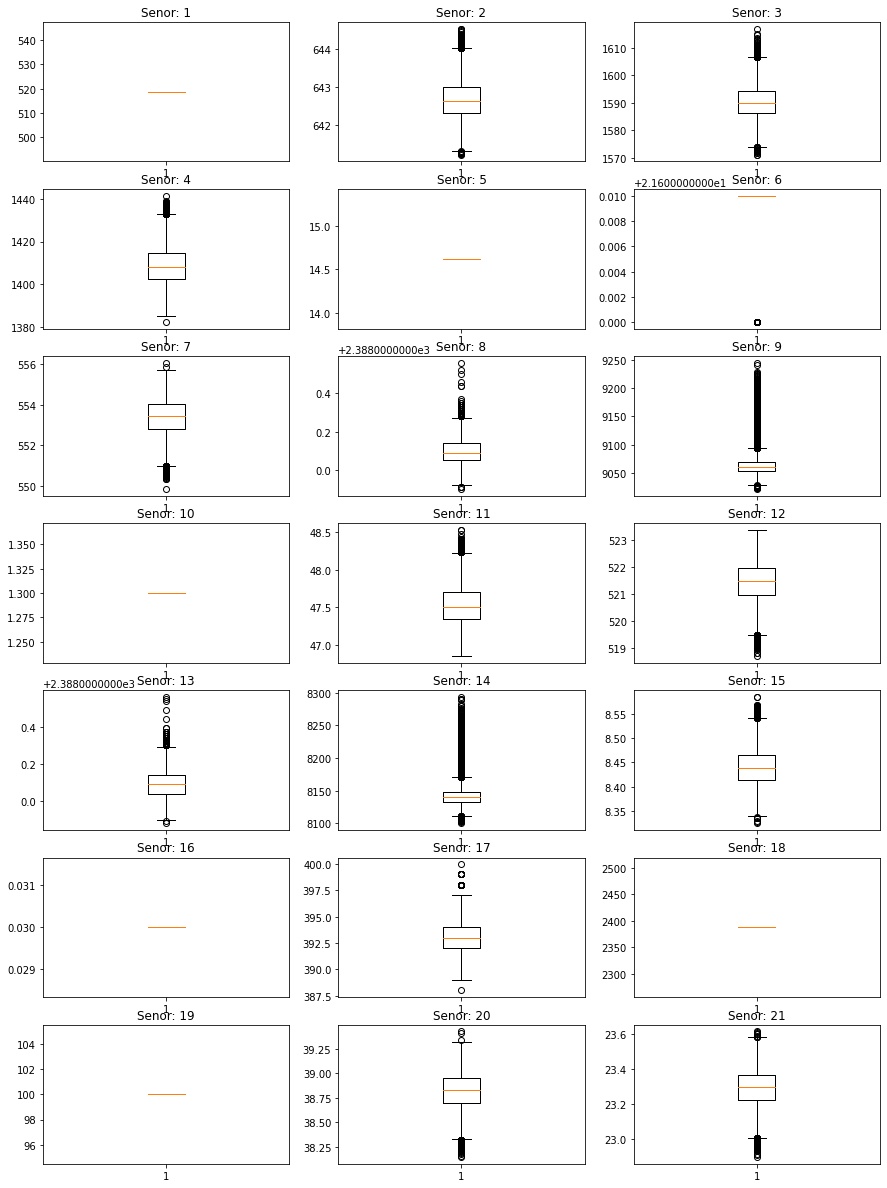
\includegraphics[width=0.85\textwidth]{preprocessing_cell27_out0.png}
    \caption{Diagrammes en boîte des mesures des 21 capteurs sur le jeu d'entraînement FD001.}
    \label{fig:boxplot_sensors}
\end{figure}

Cette visualisation met en évidence que certains capteurs présentent une variabilité quasi nulle. Une analyse plus fine révèle que les colonnes 6, 10, 15, 21, 23 et 24 contiennent des valeurs constantes (ou quasi constantes, comme la colonne 11 qui oscille entre 21,60 et 21,61). Ces capteurs ne contribuent pas à l'information utile et sont écartés du processus d'apprentissage.

\subsection{Sélection des capteurs pertinents}

Après élimination des capteurs constants, 14 capteurs sont retenus pour l'entraînement des modèles. La Figure~\ref{fig:kde_train} illustre la distribution des valeurs de ces capteurs sur le jeu d'entraînement sous forme d'estimations par noyau (KDE).

\begin{figure}[H]
    \centering
    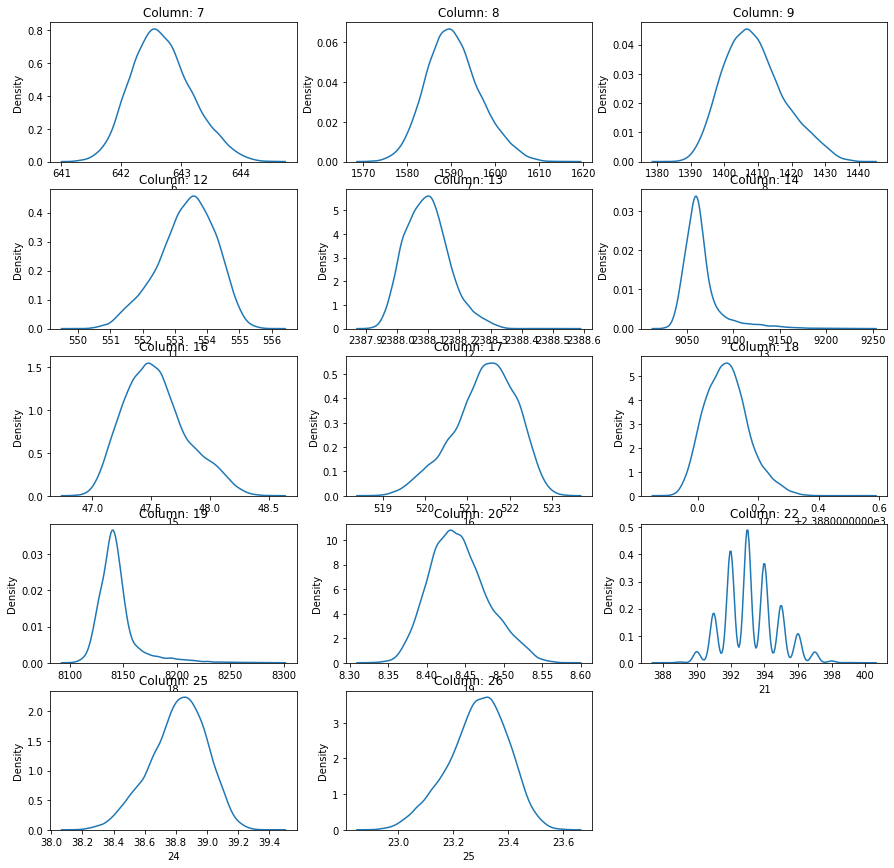
\includegraphics[width=0.85\textwidth]{preprocessing_cell31_out0.png}
    \caption{Distributions des 14 capteurs retenus sur le jeu d'entraînement FD001 (estimation par noyau).}
    \label{fig:kde_train}
\end{figure}

\subsection{Similarité entre données d'entraînement et de test}

Afin de s'assurer que les modèles pourront généraliser correctement, il est essentiel de vérifier que la distribution des données de test est similaire à celle des données d'entraînement. La Figure~\ref{fig:kde_compare} superpose les distributions des 14 capteurs pour les deux jeux de données.

\begin{figure}[H]
    \centering
    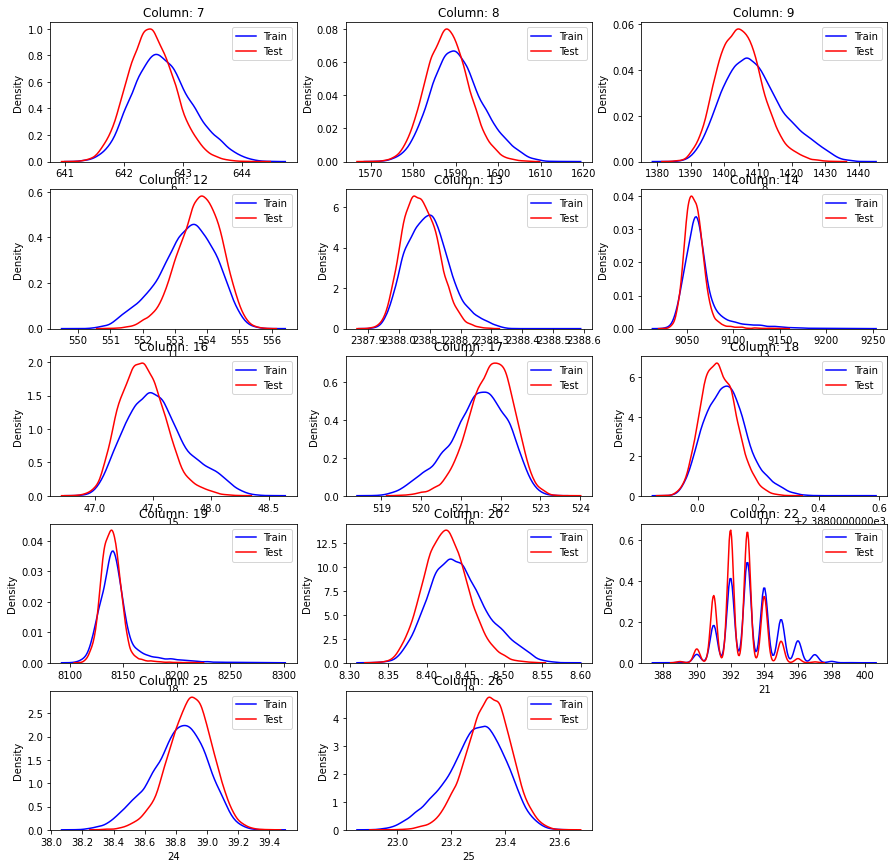
\includegraphics[width=0.85\textwidth]{preprocessing_cell33_out0.png}
    \caption{Comparaison des distributions des capteurs entre les jeux d'entraînement (bleu) et de test (orange).}
    \label{fig:kde_compare}
\end{figure}

Bien que non identiques, les distributions des données de test présentent une allure globale comparable à celles des données d'entraînement. Cette similitude constitue une condition favorable à la bonne généralisation des modèles.

\section{Modélisation de la dégradation}

Le jeu de données ne fournit pas directement les valeurs de RUL pour l'ensemble d'entraînement. Celles-ci doivent être déduites du nombre total de cycles de fonctionnement de chaque moteur.

\subsection{Modèle de dégradation linéaire}

Dans le modèle de dégradation linéaire, la RUL décroît uniformément d'une unité à chaque cycle. Si un moteur échoue après $T$ cycles, sa RUL au cycle $t$ vaut :
\begin{equation}
    \text{RUL}(t) = T - t
\end{equation}

Ainsi, au premier cycle, la RUL vaut $T-1$, et elle atteint 0 au moment de la défaillance. La Figure~\ref{fig:degradation_models} (gauche) illustre cette décroissance linéaire pour le moteur 1 du jeu FD001.

\subsection{Modèle de dégradation linéaire par morceaux}

Le modèle linéaire par morceaux (\emph{piecewise linear degradation model}) constitue une variante largement utilisée dans la littérature pour améliorer les performances de prédiction. Dans ce modèle, toute valeur de RUL supérieure à un seuil prédéfini (noté \emph{early RUL}) est plafonnée à ce seuil.

Formellement, pour un moteur ayant une durée de vie totale $T$ et un seuil $R_{\text{early}}$ :
\begin{equation}
    \text{RUL}(t) = 
    \begin{cases}
        R_{\text{early}} & \text{si } T - t > R_{\text{early}} \\
        T - t & \text{sinon}
    \end{cases}
\end{equation}

Dans ce projet, nous utilisons une valeur de $R_{\text{early}} = 125$ pour le sous-ensemble FD001. La Figure~\ref{fig:degradation_models} compare les deux modèles de dégradation pour les moteurs 1 et 7.

\begin{figure}[H]
    \centering
    \begin{subfigure}[b]{0.48\textwidth}
        \centering
        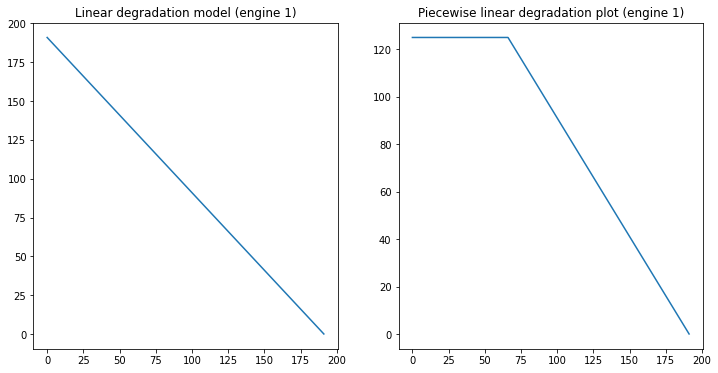
\includegraphics[width=\textwidth]{preprocessing_cell11_out0.png}
        \caption{Moteur 1 (192 cycles).}
    \end{subfigure}
    \hfill
    \begin{subfigure}[b]{0.48\textwidth}
        \centering
        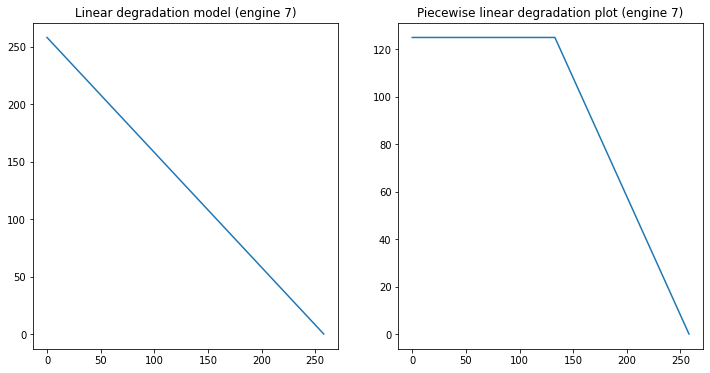
\includegraphics[width=\textwidth]{preprocessing_cell15_out0.png}
        \caption{Moteur 7 (259 cycles).}
    \end{subfigure}
    \caption{Comparaison entre le modèle de dégradation linéaire (gauche) et le modèle linéaire par morceaux avec $R_{\text{early}} = 125$ (droite).}
    \label{fig:degradation_models}
\end{figure}

\section{Fenêtrage des données temporelles}

\subsection{Principe du fenêtrage glissant}

Les données CMAPSS étant de nature temporelle, il est nécessaire de structurer les entrées des modèles sous forme de fenêtres temporelles. Le principe consiste à définir une longueur de fenêtre $W$ et un décalage $S$ (\emph{shift}) entre deux fenêtres consécutives.

Pour une séquence de $N$ observations et une fenêtre de longueur $W$, le nombre de fenêtres générées est donné par :
\begin{equation}
    B = \left\lfloor \frac{N - W}{S} \right\rfloor + 1
\end{equation}

Lorsque le décalage $S = 1$, il existe un chevauchement maximal de $W-1$ observations entre deux fenêtres successives. Dans ce projet, nous utilisons une longueur de fenêtre $W = 30$ avec un décalage $S = 1$.

\subsection{Traitement des données de test}

Pour les données de test, plusieurs stratégies sont envisageables. Nous adoptons ici une approche consistant à extraire les $N_{\text{test}}$ dernières fenêtres disponibles pour chaque moteur. La prédiction finale de la RUL est obtenue en moyennant les prédictions sur ces $N_{\text{test}}$ fenêtres, pondérées uniformément.

\subsection{Normalisation}

Avant l'entraînement, les données sont normalisées. Deux stratégies sont possibles :
\begin{itemize}
    \item \textbf{Normalisation par moteur :} Chaque moteur est normalisé individuellement à l'aide des paramètres (moyenne et écart-type, ou min et max) calculés sur ses propres données d'entraînement. Les données de test du même moteur sont ensuite normalisées avec ces mêmes paramètres.
    \item \textbf{Normalisation globale :} L'ensemble du jeu d'entraînement est normalisé conjointement, puis les données de test le sont avec les paramètres globaux.
\end{itemize}

Dans ce projet, nous utilisons principalement la normalisation \texttt{MinMaxScaler} avec une plage $[-1, 1]$ appliquée individuellement par moteur.

\section{Synthèse du pipeline de prétraitement}

Le pipeline de prétraitement complet peut être résumé comme suit :
\begin{enumerate}
    \item Chargement des fichiers bruts (train, test, RUL).
    \item Construction des cibles RUL selon le modèle linéaire par morceaux ($R_{\text{early}} = 125$).
    \item Suppression des colonnes non informatives (numéro de moteur, numéro de cycle, réglages opérationnels, capteurs constants).
    \item Normalisation MinMax par moteur sur les 14 capteurs retenus.
    \item Fenêtrage glissant des séquences avec $W = 30$ et $S = 1$.
    \item Extraction des dernières fenêtres de test pour la prédiction.
\end{enumerate}

Ce pipeline génère des tenseurs de forme $(B, 30, 14)$ pour l'entraînement, où $B$ est le nombre total de fenêtres.

% ==================== CHAPITRE 3 ====================
\chapter{Modèles de prédiction et résultats expérimentaux}\label{chap:modeles}

\section{Métriques d'évaluation}

L'évaluation des modèles de prédiction de la RUL repose sur deux métriques principales, couramment employées dans la littérature sur le jeu de données CMAPSS.

\subsection{Erreur quadratique moyenne (RMSE)}

L'erreur quadratique moyenne (Root Mean Square Error, RMSE) est définie par :
\begin{equation}
    \text{RMSE} = \sqrt{\frac{1}{N} \sum_{i=1}^{N} (y_i - \hat{y}_i)^2}
\end{equation}
où $y_i$ est la RUL réelle du moteur $i$, $\hat{y}_i$ sa RUL prédite, et $N$ le nombre total de moteurs dans le jeu de test.

La RMSE pénalise de manière quadratique les écarts entre prédictions et valeurs réelles, ce qui la rend sensible aux erreurs de grande amplitude. Elle constitue la métrique principale de comparaison entre les différentes approches.

\subsection{Score asymétrique (S-score)}

Le S-score est une métrique asymétrique qui pénalise davantage les surestimations de la RUL (prédire que le moteur durera plus longtemps qu'il ne le fait réellement) que les sous-estimations. Cette asymétrie reflète le coût plus élevé d'une défaillance imprévue par rapport à une maintenance prématurée.

Le S-score est défini par :
\begin{equation}
    S = \sum_{i=1}^{N} s_i
\end{equation}
où
\begin{equation}
    s_i = 
    \begin{cases}
        e^{-\frac{d_i}{13}} - 1 & \text{si } d_i < 0 \\
        e^{\frac{d_i}{10}} - 1 & \text{si } d_i \geq 0
    \end{cases}
\end{equation}
avec $d_i = y_i - \hat{y}_i$ l'erreur de prédiction pour le moteur $i$.

\section{Modèle XGBoost}

\subsection{Principe de l'algorithme}

XGBoost (eXtreme Gradient Boosting) est une implémentation optimisée de l'algorithme de gradient boosting sur des arbres de décision. Le principe consiste à construire séquentiellement un ensemble d'arbres de décision faibles, chaque nouvel arbre cherchant à corriger les erreurs résiduelles du modèle courant.

La fonction objectif à minimiser s'écrit :
\begin{equation}
    \mathcal{L}(\phi) = \sum_{i=1}^{N} l(y_i, \hat{y}_i) + \sum_{k=1}^{K} \Omega(f_k)
\end{equation}
où $l$ est la fonction de perte (erreur quadratique dans notre cas), $\Omega$ un terme de régularisation pénalisant la complexité de chaque arbre $f_k$, et $K$ le nombre total d'arbres.

\subsection{Préparation des données}

Contrairement au modèle LSTM qui traite des fenêtres temporelles tridimensionnelles, le modèle XGBoost requiert des entrées bidimensionnelles. Les fenêtres de forme $(B, 30, 14)$ sont donc aplaties en vecteurs de dimension $30 \times 14 = 420$.

\subsection{Entraînement et validation croisée}

L'entraînement initial est réalisé avec les hyperparamètres par défaut : \texttt{max\_depth = 3}, \texttt{learning\_rate (eta) = 1}, et 300 rounds de boosting. La Figure~\ref{fig:xgboost_train} présente l'évolution de l'erreur RMSE sur le jeu d'entraînement au cours des itérations.

\begin{figure}[H]
    \centering
    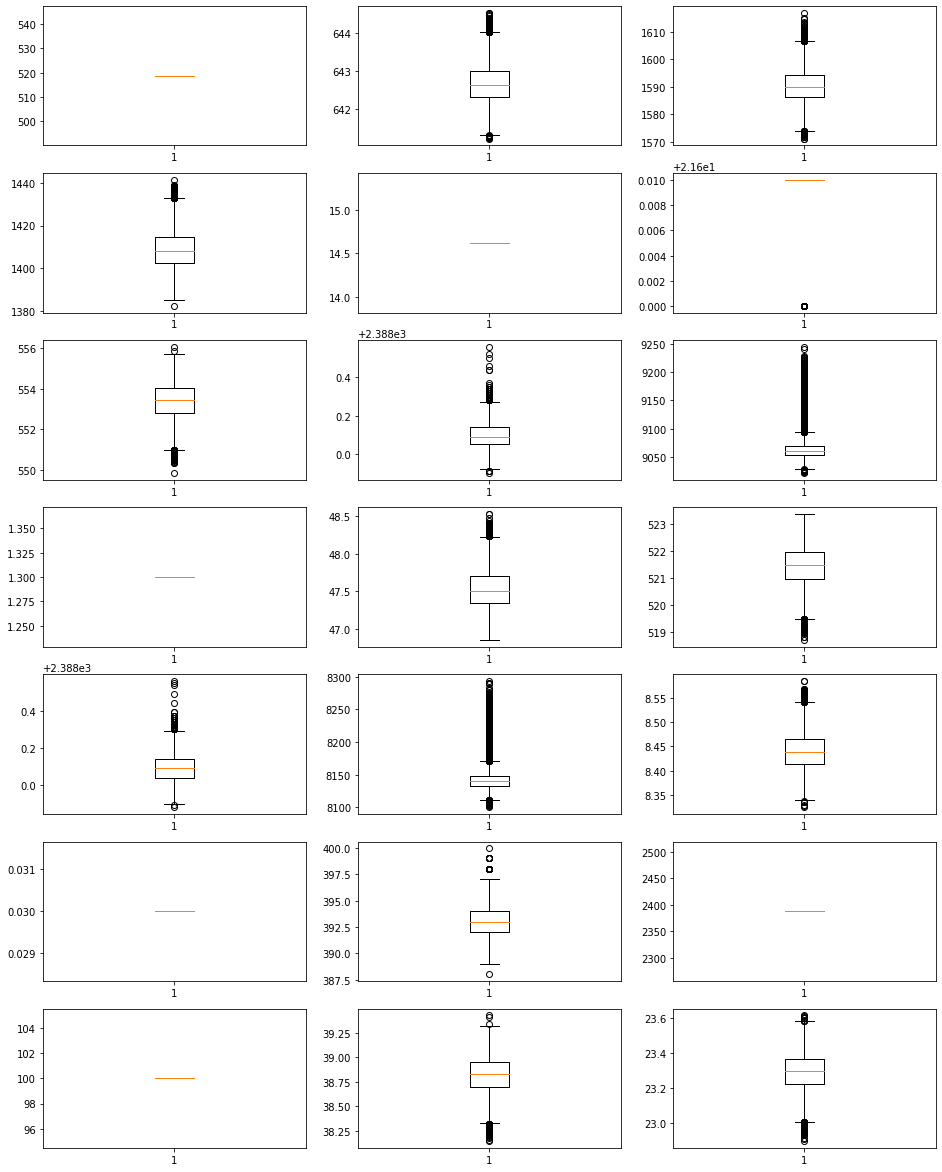
\includegraphics[width=0.75\textwidth]{xgboost_cell4_out0.png}
    \caption{Diagrammes en boîte des capteurs utilisés pour le modèle XGBoost (équivalent au prétraitement).}
    \label{fig:xgboost_train}
\end{figure}

Une recherche d'hyperparamètres par validation croisée (10 folds) est ensuite menée sur une grille couvrant différentes valeurs de \texttt{max\_depth} (de 2 à 5) et de \texttt{eta} (0,01 ; 0,1 ; 0,3 ; 0,5 ; 1,0). Le Tableau~\ref{tab:xgboost_cv} présente un extrait des résultats de cette validation croisée.

\begin{table}[H]
    \centering
    \caption{Résultats de la validation croisée pour la recherche d'hyperparamètres XGBoost (extrait).}
    \label{tab:xgboost_cv}
    \begin{tabular}{ccccl}
        \toprule
        \texttt{max\_depth} & \texttt{eta} & Meilleur RMSE & Rounds optimaux \\
        \midrule
        2 & 0,01 & 20,23 & 300 \\
        2 & 0,1  & 18,26 & 299 \\
        2 & 0,3  & 18,35 & 198 \\
        3 & 0,1  & 18,18 & 183 \\
        3 & 0,3  & 18,36 & 93  \\
        4 & 0,1  & 18,09 & 113 \\
        4 & 0,3  & 18,36 & 42  \\
        5 & 0,1  & \textbf{17,96} & 95  \\
        \bottomrule
    \end{tabular}
\end{table}

Les meilleurs hyperparamètres identifiés sont \texttt{max\_depth = 5} et \texttt{eta = 0,1}, conduisant à un RMSE de validation de 17,96 cycles. Le modèle final est entraîné avec ces paramètres sur 100 rounds.

\subsection{Résultats expérimentaux}

Le Tableau~\ref{tab:xgboost_results} synthétise les performances du modèle XGBoost sur le sous-ensemble FD001.

\begin{table}[H]
    \centering
    \caption{Performances du modèle XGBoost sur FD001 (dégradation linéaire par morceaux, $R_{\text{early}} = 125$).}
    \label{tab:xgboost_results}
    \begin{tabular}{lcc}
        \toprule
        \textbf{Configuration} & \textbf{RMSE (cycles)} & \textbf{S-score} \\
        \midrule
        Paramètres par défaut (300 rounds) & 19,78 & -- \\
        Après recherche d'hyperparamètres & 19,07 & 1~024,43 \\
        Dernière fenêtre uniquement & 18,44 & -- \\
        \bottomrule
    \end{tabular}
\end{table}

La Figure~\ref{fig:xgboost_pred} compare les valeurs réelles de RUL avec les valeurs prédites par le modèle XGBoost optimisé pour chacun des 100 moteurs du jeu de test.

\begin{figure}[H]
    \centering
    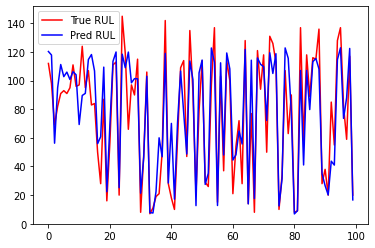
\includegraphics[width=0.85\textwidth]{xgboost_cell30_out0.png}
    \caption{Comparaison entre la RUL réelle (rouge) et la RUL prédite (bleu) par le modèle XGBoost sur le jeu de test FD001.}
    \label{fig:xgboost_pred}
\end{figure}

\subsection{Importance des variables}

L'analyse de l'importance des variables (Figure~\ref{fig:xgboost_importance}) révèle que certaines caractéristiques issues des capteurs contribuent davantage à la prédiction que d'autres. Cette information est précieuse pour comprendre quels signaux sont les plus indicatifs de l'état de dégradation du moteur.

\begin{figure}[H]
    \centering
    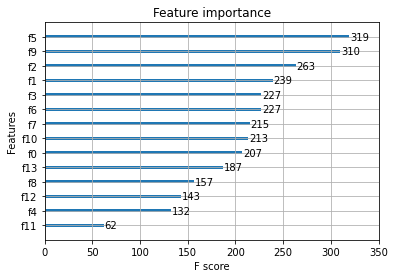
\includegraphics[width=0.85\textwidth]{xgboost_cell32_out1.png}
    \caption{Importance des variables (score F) pour le modèle XGBoost optimisé.}
    \label{fig:xgboost_importance}
\end{figure}

\section{Modèle LSTM}

\subsection{Architecture du réseau}

Le modèle LSTM implémenté est un réseau séquentiel composé de trois couches LSTM empilées suivies de deux couches denses (fully connected). L'architecture détaillée est la suivante :

\begin{itemize}
    \item \textbf{Couche LSTM 1 :} 128 neurones, activation \texttt{tanh}, retour de séquences.
    \item \textbf{Couche LSTM 2 :} 64 neurones, activation \texttt{tanh}, retour de séquences.
    \item \textbf{Couche LSTM 3 :} 32 neurones, activation \texttt{tanh}.
    \item \textbf{Couche Dense 1 :} 96 neurones, activation \texttt{ReLU}.
    \item \textbf{Couche Dense 2 :} 128 neurones, activation \texttt{ReLU}.
    \item \textbf{Couche de sortie :} 1 neurone (prédiction scalaire de la RUL).
\end{itemize}

La forme d'entrée du réseau est $(30, 14)$, correspondant à une fenêtre temporelle de 30 cycles sur 14 capteurs. Le modèle compte au total 223~521 paramètres entraînables.

\subsection{Protocole d'entraînement}

Le modèle est compilé avec la fonction de perte MSE (Mean Squared Error) et l'optimiseur Adam avec un taux d'apprentissage initial de $10^{-3}$. Un programmeur de taux d'apprentissage (\emph{Learning Rate Scheduler}) réduit ce taux à $10^{-4}$ après 5 époques.

Les données d'entraînement sont partitionnées en un jeu d'entraînement (80\%) et un jeu de validation (20\%) par échantillonnage aléatoire. L'entraînement se déroule sur 10 époques avec une taille de batch de 128. Le Tableau~\ref{tab:lstm_training} détaille l'évolution de la perte au cours de l'entraînement.

\begin{table}[H]
    \centering
    \caption{Historique d'entraînement du modèle LSTM sur FD001.}
    \label{tab:lstm_training}
    \begin{tabular}{ccccc}
        \toprule
        \textbf{Époque} & \textbf{Taux d'apprentissage} & \textbf{Perte train} & \textbf{Perte validation} \\
        \midrule
        1 & $10^{-3}$ & 3~235,05 & 959,35 \\
        2 & $10^{-3}$ & 767,49 & 604,61 \\
        3 & $10^{-3}$ & 441,49 & 309,64 \\
        4 & $10^{-3}$ & 262,40 & 235,73 \\
        5 & $10^{-3}$ & 209,63 & 169,34 \\
        6 & $10^{-4}$ & 166,29 & 161,61 \\
        7 & $10^{-4}$ & 161,67 & 161,63 \\
        8 & $10^{-4}$ & 157,90 & 154,43 \\
        9 & $10^{-4}$ & 154,89 & 151,19 \\
        10 & $10^{-4}$ & 153,65 & 149,79 \\
        \bottomrule
    \end{tabular}
\end{table}

On observe une diminution rapide de la perte durant les cinq premières époques, suivie d'une convergence plus douce après la réduction du taux d'apprentissage. Notons que l'entraînement est volontairement limité à 10 époques afin d'éviter le surapprentissage sur le jeu de validation, phénomène observé lors d'entraînements plus prolongés.

\subsection{Résultats expérimentaux}

Le Tableau~\ref{tab:lstm_results} présente les performances du modèle LSTM sur le sous-ensemble FD001.

\begin{table}[H]
    \centering
    \caption{Performances du modèle LSTM sur FD001 (dégradation linéaire par morceaux, $R_{\text{early}} = 125$).}
    \label{tab:lstm_results}
    \begin{tabular}{lcc}
        \toprule
        \textbf{Configuration} & \textbf{RMSE (cycles)} & \textbf{S-score} \\
        \midrule
        Moyenne sur les dernières fenêtres & 15,17 & -- \\
        Dernière fenêtre uniquement & 15,13 & -- \\
        S-score global & -- & 448,44 \\
        \bottomrule
    \end{tabular}
\end{table}

La Figure~\ref{fig:lstm_pred} compare les valeurs réelles et prédites de la RUL pour chaque moteur du jeu de test.

\begin{figure}[H]
    \centering
    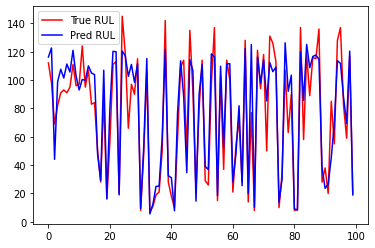
\includegraphics[width=0.85\textwidth]{lstm_cell28_out0.png}
    \caption{Comparaison entre la RUL réelle (rouge) et la RUL prédite (bleu) par le modèle LSTM sur le jeu de test FD001.}
    \label{fig:lstm_pred}
\end{figure}

Le modèle LSTM parvient à suivre avec une bonne fidélité l'évolution de la RUL réelle, avec des écarts notables pour certains moteurs présentant des comportements de dégradation atypiques.

\subsection{Sauvegarde du modèle}

Afin de garantir la reproductibilité des résultats, le modèle entraîné est sauvegardé au format HDF5 (\texttt{.h5}) sous le nom :
\begin{center}
    \texttt{FD001\_LSTM\_piecewise\_RMSE\_15.1655.h5}
\end{center}
Ce fichier de poids, d'une taille d'environ 3~MB, peut être rechargé dans un environnement TensorFlow pour effectuer de nouvelles inférences sans nécessiter de réentraînement.

\section{Comparaison des performances}

\subsection{Tableau comparatif}

Le Tableau~\ref{tab:comparison} synthétise les performances des deux modèles sur le sous-ensemble FD001 avec le modèle de dégradation linéaire par morceaux ($R_{\text{early}} = 125$).

\begin{table}[H]
    \centering
    \caption{Comparaison des performances entre XGBoost et LSTM sur FD001.}
    \label{tab:comparison}
    \begin{tabular}{lcc}
        \toprule
        \textbf{Métrique} & \textbf{XGBoost} & \textbf{LSTM} \\
        \midrule
        RMSE (cycles) & 19,07 & \textbf{15,17} \\
        S-score & 1~024,43 & \textbf{448,44} \\
        Nombre de paramètres & -- & 223~521 \\
        Temps d'entraînement & Quelques secondes & $\approx$ 100 secondes \\
        \bottomrule
    \end{tabular}
\end{table}

\subsection{Analyse des résultats}

Les résultats expérimentaux mettent en évidence la supériorité du modèle LSTM sur le modèle XGBoost pour ce problème de prédiction de la RUL :

\begin{itemize}
    \item \textbf{Précision :} Le LSTM réduit l'erreur RMSE de près de 4 cycles (soit une amélioration relative de 20,4\%), ce qui représente une avancée significative dans le contexte aéronautique où chaque cycle compte.
    
    \item \textbf{Score asymétrique :} Le S-score du LSTM (448,44) est moins de la moitié de celui du XGBoost (1~024,43), indiquant que le réseau de neurones récurrent commet moins d'erreurs de surestimation coûteuses.
    
    \item \textbf{Capacité de modélisation temporelle :} Cette supériorité s'explique par la capacité intrinsèque des LSTM à capturer les dépendances séquentielles dans les données de dégradation. Alors que le XGBoost traite chaque fenêtre comme un vecteur statique indépendant, le LSTM exploite explicitement la dimension temporelle.
    
    \item \textbf{Complexité et ressources :} Cette meilleure performance s'accompagne cependant d'une complexité accrue. Le modèle LSTM compte plus de 220~000 paramètres et nécessite un temps d'entraînement d'environ 100 secondes, contre quelques secondes seulement pour XGBoost.
\end{itemize}

\subsection{Discussion}

Il convient de souligner que le choix entre XGBoost et LSTM dépend du contexte opérationnel. Si la précision de prédiction est primordiale et que les ressources de calcul sont disponibles, le LSTM constitue le meilleur choix. En revanche, pour des applications nécessitant une interprétabilité élevée ou un temps d'entraînement minimal, XGBoost reste une solution très compétitive.

Par ailleurs, la nature non déterministe de certaines opérations en apprentissage profond (notamment dans les bibliothèques comme TensorFlow) peut conduire à de légères variations des résultats selon l'architecture matérielle utilisée. C'est pourquoi le projet fournit les poids du modèle pré-entraîné, garantissant ainsi une reproductibilité exacte des performances annoncées.

% ==================== CHAPITRE 4 ====================
\chapter{Application de démonstration Streamlit}\label{chap:demo}

\section{Objectifs de l'application}

Afin de démontrer la pertinence pratique des modèles développés, une application interactive a été conçue à l'aide de la bibliothèque Streamlit. Cette application vise à :
\begin{itemize}
    \item Permettre l'interaction avec le modèle LSTM pré-entraîné sans nécessiter de connaissances techniques approfondies.
    \item Visualiser en temps réel les prédictions de RUL sur un sous-ensemble du jeu de test.
    \item Afficher les métriques de performance et les courbes d'apprentissage du modèle.
    \item Offrir une comparaison visuelle entre la RUL réelle et la RUL prédite.
\end{itemize}

\section{Architecture de l'application}

L'application est structurée autour de plusieurs onglets (ou sections) accessibles depuis une barre latérale :

\subsection{Page d'accueil}

La page d'accueil présente le contexte du projet, une description du jeu de données CMAPSS et les objectifs de l'application. Elle oriente l'utilisateur vers les différentes fonctionnalités disponibles.

\subsection{Prédiction interactive}

Cette section constitue le coeur de l'application. Elle permet à l'utilisateur de :
\begin{itemize}
    \item Sélectionner un moteur spécifique parmi les 100 moteurs du jeu de test FD001.
    \item Choisir le nombre de fenêtres temporelles à extraire pour la prédiction.
    \item Visualiser les signaux des capteurs du moteur sélectionné.
    \item Obtenir la prédiction de la RUL accompagnée d'un intervalle de confiance estimé.
\end{itemize}

Le modèle LSTM sauvegardé (\texttt{FD001\_LSTM\_piecewise\_RMSE\_15.1655.h5}) est chargé en mémoire via TensorFlow. Les données de test sont prétraitées à la volée selon le même pipeline que celui décrit dans le Chapitre~\ref{chap:donnees}.

\subsection{Métriques et performance}

Cette section affiche un tableau de bord complet des performances du modèle :
\begin{itemize}
    \item Valeurs de la RMSE et du S-score sur l'ensemble du jeu de test.
    \item Historique de la perte (courbes d'entraînement et de validation) récupéré depuis le notebook LSTM.
    \item Matrice d'erreur $d_i = y_i - \hat{y}_i$ pour chaque moteur, avec mise en évidence des surestimations et sous-estimations.
\end{itemize}

\subsection{Visualisation comparative}

La visualisation la plus illustrative est la comparaison graphique entre la RUL réelle et la RUL prédite. L'application génère un graphique similaire à la Figure~\ref{fig:lstm_pred}, avec des options d'interaction (zoom, sélection de moteurs, affichage de la bande d'erreur $\pm$ RMSE).

\subsection{Comparaison XGBoost vs LSTM}

Une section dédiée juxtapose les prédictions des deux modèles pour le même sous-ensemble de moteurs. Un graphique superposé permet d'apprécier visuellement la meilleure adéquation du LSTM aux valeurs réelles, particulièrement pour les moteurs présentant des profils de dégradation complexes.

\section{Technologies utilisées}

L'application repose sur les technologies et bibliothèques suivantes :
\begin{itemize}
    \item \textbf{Streamlit :} Framework Python pour la création rapide d'applications web de data science.
    \item \textbf{TensorFlow / Keras :} Chargement et inférence du modèle LSTM pré-entraîné.
    \item \textbf{NumPy / Pandas :} Manipulation des données et prétraitement.
    \item \textbf{Matplotlib / Plotly :} Visualisations interactives et statiques.
\end{itemize}

\section{Intérêt pédagogique}

Cette application de démonstration présente un double intérêt pédagogique. D'une part, elle matérialise les concepts théoriques abordés dans ce rapport en les rendant interactifs et accessibles. D'autre part, elle illustre la chaîne complète de déploiement d'un modèle d'apprentissage automatique, depuis la phase de recherche (notebooks Jupyter) jusqu'à la mise à disposition d'un outil utilisable par un non-spécialiste.

% ==================== CONCLUSION ====================
\chapter*{Conclusion générale}
\addcontentsline{toc}{chapter}{Conclusion générale}

Ce projet de fin de module a permis d'explorer en profondeur le domaine de la prédiction data-driven de la Vie Utile Résiduelle (RUL), à travers l'étude du jeu de données CMAPSS de la NASA. En nous appuyant sur une démarche rigoureuse de prétraitement des données et sur l'implémentation de deux modèles représentatifs -- XGBoost et LSTM -- nous avons pu comparer quantitativement les mérites respectifs des approches classiques et profondes.

Les principaux enseignements tirés de ce travail sont les suivants :

\begin{enumerate}
    \item \textbf{Importance du prétraitement :} La qualité de la prédiction dépend crucialement de la pertinence du pipeline de prétraitement. L'élimination des capteurs non informatifs, la normalisation appropriée et le choix du modèle de dégradation constituent des étapes déterminantes.
    
    \item \textbf{Supériorité des réseaux récurrents :} Sur le sous-ensemble FD001, le modèle LSTM surpasse significativement le modèle XGBoost, avec une réduction de l'erreur RMSE de 20,4\% (de 19,07 à 15,17 cycles) et un S-score divisé par plus de deux. Cette amélioration s'explique par la capacité du LSTM à modéliser explicitement les dépendances temporelles dans les séquences de dégradation.
    
    \item \textbf{Reproductibilité :} La démarche adoptée, consistant à documenter chaque étape dans des notebooks Jupyter et à archiver les modèles pré-entraînés, garantit la transparence et la reproductibilité des résultats obtenus.
    
    \item \textbf{Passage à l'échelle opérationnelle :} L'application Streamlit de démonstration illustre la faisabilité du déploiement de tels modèles dans un contexte industriel, tout en soulignant les défis liés à l'interprétabilité et à la confiance des opérateurs dans les prédictions automatisées.
\end{enumerate}

\section*{Perspectives}
\addcontentsline{toc}{section}{Perspectives}

Plusieurs pistes d'amélioration et d'extension de ce travail peuvent être envisagées :

\begin{itemize}
    \item \textbf{Exploitation des autres sous-ensembles :} Les sous-ensembles FD002, FD003 et FD004 présentent des conditions opérationnelles et des modes de défaillance variés. Leur analyse permettrait d'évaluer la robustesse des modèles face à une plus grande diversité de scénarios.
    
    \item \textbf{Mécanismes d'attention :} L'intégration de mécanismes d'attention (comme l'attention additive couplée à des GRU) a démontré dans la littérature et dans le projet original des gains supplémentaires significatifs (RMSE de 14,21 sur FD001).
    
    \item \textbf{Approches hybrides :} La combinaison de modèles physiques simplifiés avec des modèles data-driven pourrait améliorer la généralisation et l'interprétabilité des prédictions.
    
    \item \textbf{Prédiction probabiliste :} Au lieu de prédire une valeur ponctuelle de RUL, l'estimation d'une distribution de probabilité (par exemple via des réseaux bayésiens ou des méthodes d'ensemble) fournirait une information plus riche pour la prise de décision de maintenance.
    
    \item \textbf{Déploiement embarqué :} L'optimisation et la compression du modèle LSTM (quantification, pruning) pourraient permettre son intégration directement dans les systèmes de bord des moteurs.
\end{itemize}

En conclusion, ce projet a constitué une immersion enrichissante dans les techniques modernes de pronostics industriels. Il nous a permis de maîtriser l'ensemble de la chaîne de traitement, depuis l'analyse exploratoire des données jusqu'à la mise en oeuvre de modèles d'apprentissage profond, en passant par la réflexion sur les enjeux du déploiement opérationnel.

% ==================== BIBLIOGRAPHIE ====================
\begin{thebibliography}{99}
\addcontentsline{toc}{chapter}{Bibliographie / Webographie}

\bibitem{nasa_cmapss}
NASA Prognostics Center of Excellence.
\textit{CMAPSS -- Jet Engine Simulated Data}.
Disponible sur : \url{https://data.nasa.gov/Aerospace/CMAPSS-Jet-Engine-Simulated-Data/ff5v-kuh6}

\bibitem{sahoo2020}
B. Sahoo.
\textit{Data-Driven Remaining Useful Life (RUL) Prediction}.
Projet open-source, 2020. DOI : 10.5281/zenodo.5890595.
Disponible sur : \url{https://biswajitsahoo1111.github.io/rul_codes_open/}

\bibitem{hochreiter1997}
S. Hochreiter et J. Schmidhuber.
\textit{Long Short-Term Memory}.
Neural Computation, vol. 9, no. 8, pp. 1735--1780, 1997.

\bibitem{chen2016}
T. Chen et C. Guestrin.
\textit{XGBoost: A Scalable Tree Boosting System}.
Proceedings of the 22nd ACM SIGKDD International Conference on Knowledge Discovery and Data Mining, pp. 785--794, 2016.

\bibitem{olah2015}
C. Olah.
\textit{Understanding LSTM Networks}.
Blog post, 2015.
Disponible sur : \url{https://colah.github.io/posts/2015-08-Understanding-LSTMs/}

\bibitem{d2l_attention}
A. Zhang, Z. C. Lipton, M. Li, and A. J. Smola.
\textit{Dive into Deep Learning}, Chapitre 10 : Attention Mechanisms.
Disponible sur : \url{https://classic.d2l.ai/chapter_attention-mechanisms/index.html}

\bibitem{tensorflow}
M. Abadi et al.
\textit{TensorFlow: Large-Scale Machine Learning on Heterogeneous Systems}, 2015.
Disponible sur : \url{https://www.tensorflow.org/}

\bibitem{streamlit}
Streamlit Inc.
\textit{Streamlit -- The fastest way to build and share data apps}.
Disponible sur : \url{https://streamlit.io/}

\end{thebibliography}

\end{document}
